\Problem{Suspended Loudspeaker}{\LoudHang}{
A 25 kg loudspeaker is suspended 2.0 m below the ceiling by two cables that are each 30$ ^{\circ} $ from vertical.
}
\ProblemSub{\LoudHangA}{
(a) Draw a sketch illustrating the problem.
}
\Solution{\LoudHangASol}{
\begin{figure}[h]
	\centering
	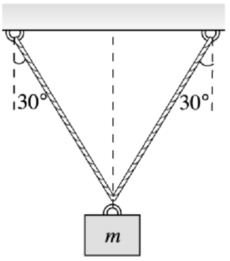
\includegraphics{\FileDepth/Activities/Suspended_Loudspeaker/Two_Cable_Speaker.pdf}
\end{figure}
}
\ProblemSub{\LoudHangB}{
(b) Draw a free-body diagram for the loudspeaker.
}
\Solution{\LoudHangBSol}{
\begin{figure}[h]
	\centering
	\begin{tikzpicture}
		\FBDaxes{0,0}{0}{axes}
		\FBDvectorMA{axes}{0.866}{60}{RT}
		\node[anchor=west] at (RTtip) {$\vec{F}^{T}_{SR}$};
		\node at (0.15,0.6) {$\theta$};
		\FBDvectorMA{axes}{0.866}{120}{LT}
		\node[anchor=east] at (LTtip) {$\vec{F}^{T}_{SL}$};
		\node at (-0.15,0.6) {$\theta$};
		\FBDvectorXY{axes}{0,-1.5}{FG}
		\node[anchor=west] at (FGtip) {$\vec{F}^{g}_{SE}$};
	\end{tikzpicture}
\end{figure}

Here, $\vec{F}^{T}_{SR}$ is the tension acting on the speaker from the cable on the right, and $\vec{F}^{T}_{SL}$ is the tension acting on the speaker from the cable on the left. Since there is only one object, I will drop the $S$ subscript in further calculations, and since there is only one force of gravity, I will drop both subscripts from it.
}
\ProblemSub{\LoudHangC}{
(c) Find the tension in each cable.
}
\Solution{\LoudHangCSol}{
First, we consider the $ x $-components. The loudspeaker is not accelerating, so
\[
F^{net}_{x} = ma_{x} = 0.
\]
The sum of the forces in this direction is
\[
F^{net}_{x} = F^{T}_{R}\sin\theta - F^{T}_{L}\sin\theta,
\]
therefore
\[
\begin{split}
	F^{T}_{L}\cancel{\sin\theta} & = F^{T}_{R}\cancel{\sin\theta} \\
	F^{T}_{L} & = F^{T}_{R}.
\end{split}
\]
This can be seen in the symmetry of the problem. Now, in the vertical direction, we have
\[
\begin{split}
	F^{net}_{y} & = ma_{y} = 0 \\
	F^{T}_{R}\cos\theta + F^{T}_{L}\cos\theta - F^{g} & = 0 \\
	2F^{T}_{R}\cos\theta - mg & = 0 \\
	F^{T}_{R} & = \frac{mg}{2\cos\theta} \\
	& = \frac{(25\text{ kg})(9.8\text{ m/s}^{2})}{2\cos(30^{\circ})} \\
	& \approx 140\text{ N}.
\end{split}
\]
Each cable has 140 N of tension in it.
}